% SIAM Shared Information Template
% This is information that is shared between the main document and any
% supplement. If no supplement is required, then this information can
% be included directly in the main document.

In this section we study the impact of parameter $\epsilon_s$ and hardware parallelism on the quality of  RACE method. \Inorder to do this we first quantify the quality of the method and finally we  use this quantity to do a parameter study. The study gives insights into tuning of parameter $\epsilon_s$ based on the given matrix and required parallelism.


\subsection{Quantifying quality of RACE}
Quantifying quality of the method in a well-defined way is a primary and most vital step for parameter study. We do this using the concept of \effPar. From \cref{Sec:race} we saw that even though one tries to achieve parallelism exactly as that required by the hardware, in practice one might not be able to utilize this parallelism to 100 \% due to load imbalances. Therefore we use a simple calculation based on the \levelTree to determine efficiency, taking into account load imbalances from different stages of recursion. So we first calculate \effRow for each of the finest leaves (worker leaves) in \levelTree. \EffRow for each worker leaf is the same as number of rows (\nrows) on which each leaf has to operate, for example in case of $T_1(0)$ \effRow (\nrowsEff$(T_1(0))$) is 14 and \nrowsEff$(T_2(0) \subset T_1(4))$ is 6. After calculating the \effRow for worker leaves the information is propagated to lower stages (up in the \levelTree) as follows: 
\begin{align*}
\nrowsEffMath(T_s(i)) &= max(\nrowsEffMath(T_{s+1}(j) \subset T_s(i))) + max(\nrowsEffMath(T_{s+1}(k) \subset T_s(i)))\\
 & \text{for } j \text{ is even and } k \text{ is odd}
\end{align*}

Such a definition for \effRow is based on the idea that a parent has to wait until the child leaf with most number of rows has finished it's work due to synchronization needed with it's siblings. This has to be handled separately for each of the two parallel sweep as there is this synchronization happening after each of the sweeps. 

Once the information is propagated up the tree and as it reaches the root we have a single \effRow (\nrowsEff$(T_0)$) for the entire tree, which has taken care of load balancing happening between all \levelGroups in all stages. The ratio of total number of rows in the entire matrix to that of \nrowsEff$(T_0)$ gives \effPar, denoted as \threadEff. Efficiency ($\eta$) of the method is then defined as ratio of  \threadEff to that of required hardware parallelism ($n\_threads$). 

\begin{align}
	\threadEffMath &= \frac{nrows}{\nrowsEffMath(T_0)} \\
	\eta &= \frac{\threadEffMath}{n\_threads} \label{eq:eta}
\end{align}

For example in our \STEX example, \cref{fig:rec_2d-7pt_tree} shows \nrowsEff for each leaves in angular brackets and here $\threadEffMath = 5.8$ and $\eta = 0.725$. The value of $\eta = 1$ implies there is perfect load balancing, else $0 < \eta \leq 1$.

This parameter $\eta$ will be used as a measure of quality in parameter study. One has to note that the efficiency ($\eta$) calculated here is a worse case scenario and in reality memory bandwidth saturation and other factors will normally lead to a better efficiency.

\subsection{Case study}
A given matrix has a fixed amount of parallelism and as the amount of required parallelism ($nthreads$) increases load balancing degrades due to more threads per stage and imbalances between stages. The rate of degradation can however be controlled to certain extent by the tolerance $\epsilon_s$ (see \cref{eq:epsilon}) specified while choosing a \levelGroup. Typical value of $\epsilon_s$ is in range of [0.4,0.9]. Having a small $\epsilon_s$ (for example 0.4) implies we utilize the current stage `s' to maximum and do not impose high load balancing constraint, a high value on the other hand requires more balanced load from current stage `s'. 

Test matrices (see \cref{Sec:test_bed}) considered have a varying degree of parallelism, and in order to see the effect of $\eta$ and $\epsilon_s$ we choose \emph{inline} matrix. The choice is due to the fact that this matrix has relatively small amount of parallelism and this allows us to demonstrate various effect, ranging from good to bad case scenario with small number of parallelism ($nthreads < 200$). This limited parallelism can be observed from \cref{fig:inline-a} 
where efficiency keeps on decreasing with $n\_threads$ for \emph{inline} matrix. Similar behavior can be observed for \emph{crankseg} and \emph{ship} matrices which we will discuss in \cref{Sec:expt}. For majority of other test matrices one could observe that efficiency $\eta$ initially drops but then remains almost constant ($\eta$ = [0.70,0.85]) for the entire scanned area of $n\_threads\leq200$.

\begin{figure}[tbhp]
	\centering
	\subfloat[$n\_threads$ vs $\eta$]{\label{fig:inline-a}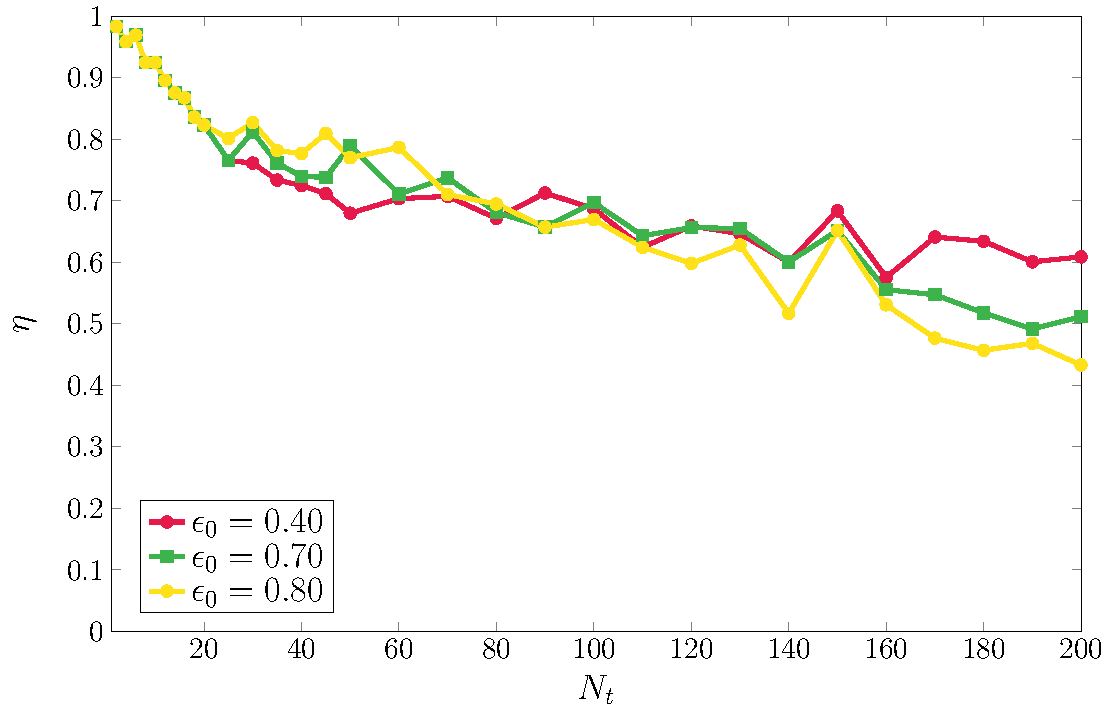
\includegraphics[width=0.45\textwidth , height=0.2\textheight]{pics/param_study/threads_vs_eff}}
	\hspace{1.5em}
	\subfloat[Effect of $\epsilon_1$ at low $nthreads$]{\label{fig:inline-b}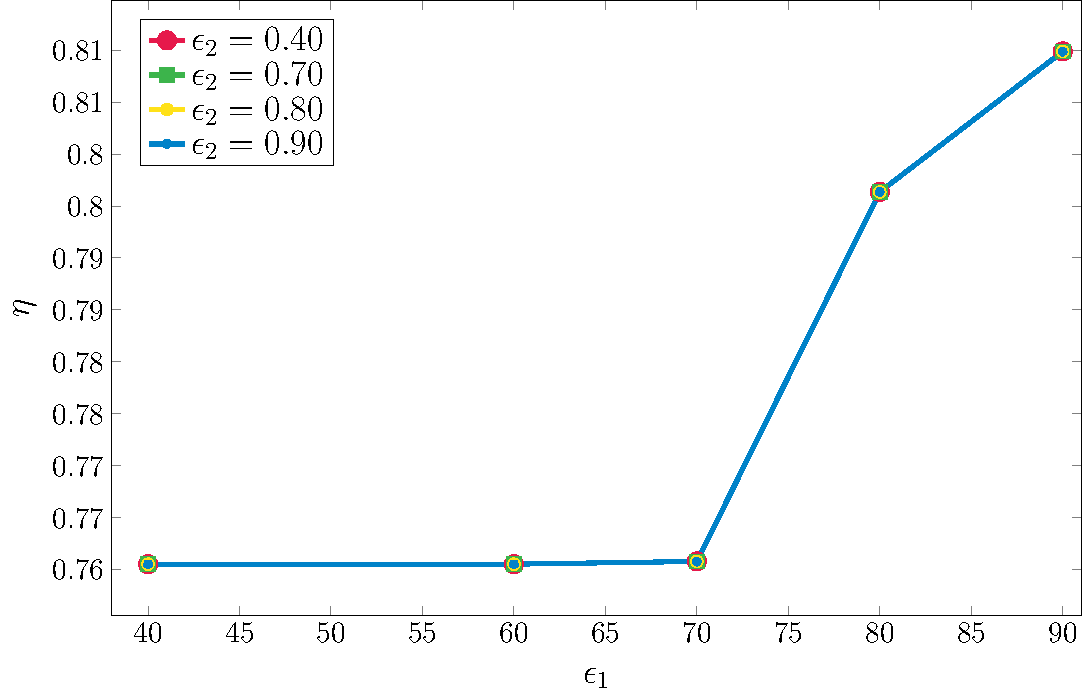
\includegraphics[width=0.45\textwidth , height=0.2\textheight]{pics/param_study/scaling_eps_1_25_threads}}
	
	\subfloat[Optimal $\epsilon_1$ lowered, optimal $\epsilon_2$ = 0.9 ]{\label{fig:inline-c}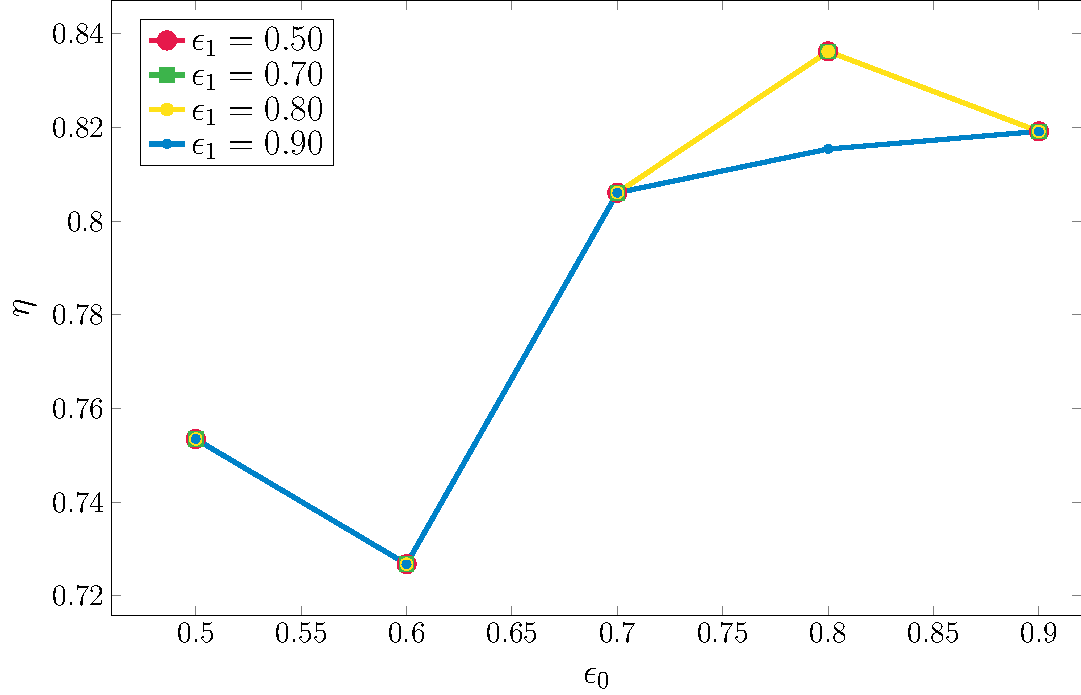
\includegraphics[width=0.45\textwidth , height=0.2\textheight]{pics/param_study/scaling_eps_1_45_threads}}
	\hspace{1.5em}
	\subfloat[Optimal $\epsilon_1$ lowered to 0.4 and $\epsilon_2$ to 0.7 ]{\label{fig:inline-d}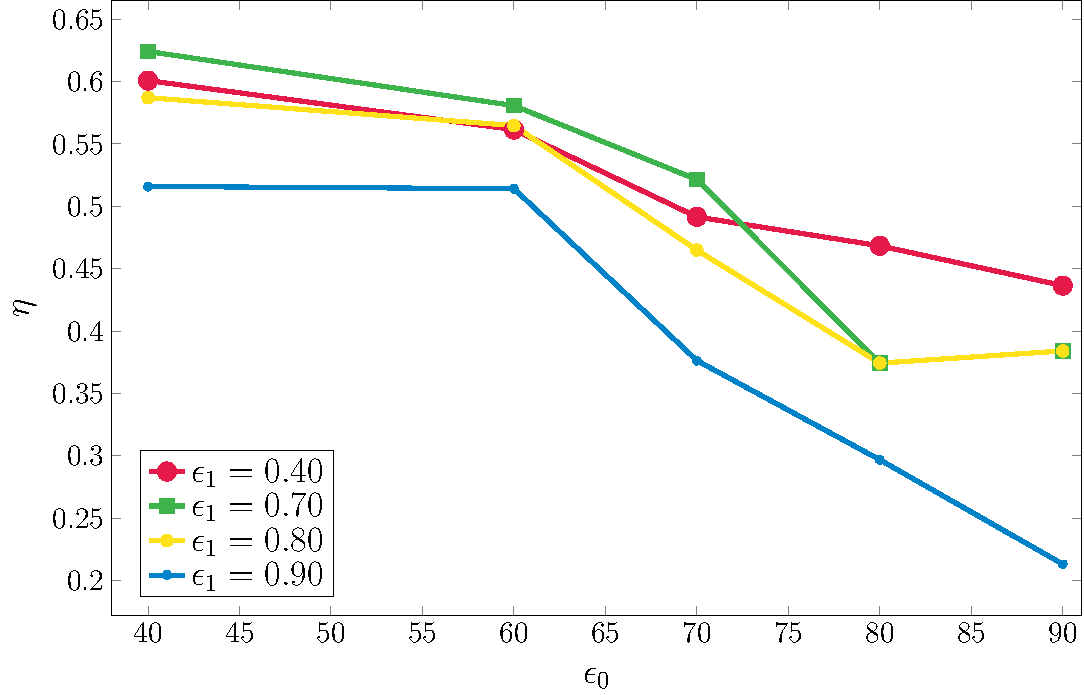
\includegraphics[width=0.45\textwidth , height=0.2\textheight]{pics/param_study/scaling_eps_1_190_threads}}
	\caption{Parameter study on \emph{inline} matrix}
	\label{fig:inline_param_study}
\end{figure}

At small number of $nthreads$ all matrices have good efficiency $\eta$. As there is a lot of parallelism in this stage compared to requirement, $\eta$ is insensitive of $\epsilon_s$. Increasing $nthreads$ one could then gradually observe $\eta$ starts to vary with $\epsilon_1$. For example in case of $nthreads = 25$ one could see in \cref{fig:inline-b} maximum $\eta$ is achieved with high value of $\epsilon_1$ (0.9) due to good load balancing. But as $nthreads$ further increase the optimal $\epsilon_1$ starts shifting towards left (see \cref{fig:inline-c}),
 since one requires more parallelism from the current stage (1) and higher $\epsilon_1$ would be decremental since it would require the \levelTree to go more deep and hence load imbalances in next stages will get multiplied. $\epsilon_2$ which till now didn't effect much starts to influence slowly as $nthreads$ increments again.For example in case of \emph{inline} till $nthreaads=90$ $\epsilon_2=0.9$ was optimal, but then the optimal $\epsilon_2$ reduces and reaches $0.7$ at $n\_threads=190$ as seen in \cref{fig:inline-d}. $\eta$ would start to get affected by $\epsilon_s$ of next stages in similar manner with increase of $n\_threads$.
 
In practice for a given matrix it's difficult to precisely determine the optimal rate of decrease in $\epsilon_s$ without parameter search, and therefore selecting proper $\epsilon_s$ for given $n\_threads$ can be challenging. One idea is to see the \totalLvl and distribution of \nrows (or \nnz) in different levels of current stage `s' and heuristically determine $\epsilon_s$ based on the pressure of parallelism from stage `s'. This is not currently done and is part of our future work. Currently for experiments we set $\epsilon_s=0.8$ for all matrices.


